La figure ci-dessous présente les équations d'état de trois gaz parfaits non relativistes à trois
dimensions (numérotées de haut en bas). Les $N$ particules de masse $m$, confinées dans un volume $V$ sont supposées sans
structure interne. Le produit $pV$ et la température $T$ sont adimensionnés grâce à la température
caractéristique : $T_0=\frac{h^2}{2\pi m k_B} \left( \frac{N}{V} \right)^{\frac{2}{3}}.$



\question
Rappeler la définition de la longueur d'onde de De Broglie $\Lambda$ à la température $T$.
Quel est son sens physique ? En déduire une interprétation de la température caractéristique $T_0$.

\question \`A quelle statistique étudiée en cours chacune de ces trois courbes correspond-elle ?

\question Expliquer l'existence d’une ordonnée à l’origine non nulle pour la courbe 1. Donner un exemple de système physique qui vérifie cette équation d'état.

\question
Concernant la courbe 3, à quel phénomène physique
la température $T^*=\frac{T_0}{\zeta(\frac{3}{2})^{\frac{2}{3}}} \approx  0,52 \ T_0$ (indiquée par un trait vertical sur la figure) correspond-elle ? $\zeta(s)=\sum_{k=1}^{+\infty} \frac{1}{k^s}$ est la fonction zêta de Riemann. 

\question Pour $T \gg T_0$, les trois courbes se rejoignent. En pratique, la courbe 2 est-elle réaliste à basse température ? Pourquoi ?

\begin{center}
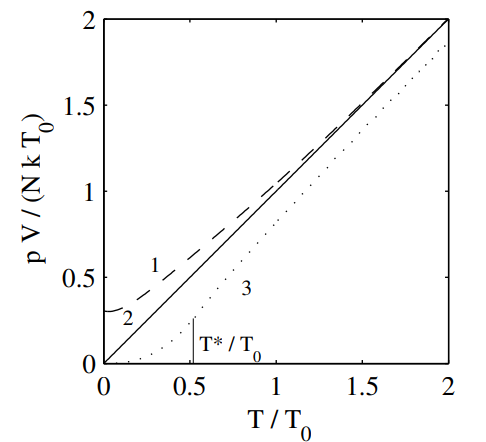
\includegraphics[scale=0.4]{../Fig/TroisStatistiques}
\end{center}
